\documentclass[UTF8,fontset=windows,11pt,a4paper]{ctexart}

\usepackage[top=2.1cm,bottom=2.1cm,left=2.25cm,right=2.25cm]{geometry}
\usepackage{amsmath,amssymb,bm}
\usepackage{booktabs}
\usepackage{graphicx,float,caption}
\usepackage{fancyhdr}
\usepackage[hidelinks]{hyperref}

\setmainfont{Times New Roman}
\setsansfont{Arial}
\setmonofont{Consolas}

\pagestyle{fancy}
\fancyhf{}
\lhead{位移反推与曲壳计算结果分析}
\rhead{2026年7月21日}
\cfoot{\thepage}
\setlength{\headheight}{14pt}
\setlength{\parindent}{2em}
\setlength{\parskip}{0.15em}
\setlength{\emergencystretch}{2em}
\renewcommand{\arraystretch}{1.12}
\captionsetup{font=small,labelfont=bf}

\title{位移反推与曲壳计算结果分析}
\author{}
\date{2026年7月21日}

\begin{document}
\maketitle

\begin{abstract}
本报告核对两项计算结果：根据给定中心位移反求加载电势和磁势，以及不同曲率圆柱壳的中心位移。逐层源项装配修正后，MATLAB 与 COMSOL 在 0.5、1.0 和 2.0~mm 三个位移目标下的相对差均约为 1.84\%。曲壳表11重新完成了 $20\times20$ 和 $30\times30$ 两级网格计算，24 组配对的最大变化为 0.007878\%，说明 MATLAB 位移对面内网格已经稳定。现有 COMSOL 曲壳模型只核对了 $R=0.4$~m 的压力工况，尚不能代表表11的全部组合。
\end{abstract}

\section{比较范围决定了数值能否直接对照}

位移反推采用线性静力关系。机械位移和温度确定后，电势与磁势由各自的耦合方程求得：
\begin{align}
  \bm K_{\phi\phi}\bm\phi
  &=-\bm K_{\phi,uT}
  \begin{bmatrix}\bm u\\\bm T\end{bmatrix},
  &
  \bm K_{\psi\psi}\bm\psi
  &=-\bm K_{\psi,uT}
  \begin{bmatrix}\bm u\\\bm T\end{bmatrix}.
\end{align}
若参考位移为 $w_0$、目标位移为 $w^*$，线性比例系数为 $s=w^*/w_0$。因此三个目标位移对应的电势和磁势严格成比例，它们用于检查线性缩放关系，不是三个相互独立的统计样本。

跨软件相对差按 MATLAB 结果归一化：
\begin{equation}
  \delta=\frac{|y_{\mathrm{COMSOL}}-y_{\mathrm{MATLAB}}|}
  {|y_{\mathrm{MATLAB}}|}\times100\%.
\end{equation}
当前比较对齐了几何、材料、边界和观测量，但 MATLAB 使用 LRT5 壳模型，COMSOL 使用三维二次实体，两者的机械离散并不相同。下文因此使用“相对差”而不是“数值误差”。

钱沈云文献中的圆柱壳算例采用 $R=0.6$~m、圆心角 $0.5$~rad 和 10~kPa 压力，考察一阶频率与受压位移。本报告的反推问题以规定中心位移为输入，输出电势和磁势。两者的几何、载荷和输出不同，不能直接要求数值相等；文献只能用于核对建模思路、边界处理和收敛方法。

\section{逐层装配修正使反推结果明显下降}

旧程序在处理一个物理层时，把该层的热释电和热释磁系数写入了全部活动势自由度。外层循环随后又遍历所有层，造成源项重复累加。修正后，每层材料只写入本层自由度，同时删除入口处按层数统一缩放的补偿。表\ref{tab:before-after}给出相同 $10\times10$ 面内网格下的变化。

\begin{table}[H]
\centering
\caption{源项装配修正前后的反推结果}
\label{tab:before-after}
\small
\begin{tabular}{rrrrrrr}
\toprule
$w^*$/mm & 旧值/V & 修正值/V & 变化/\% & 旧值/A & 修正值/A & 变化/\% \\
\midrule
0.5 & 164.544443 & 78.431689 & $-52.3340$ & 0.170287139 & 0.030880910 & $-81.8654$ \\
1.0 & 329.088887 & 156.863379 & $-52.3340$ & 0.340574277 & 0.061761819 & $-81.8654$ \\
2.0 & 658.177773 & 313.726757 & $-52.3340$ & 0.681148555 & 0.123523638 & $-81.8654$ \\
\bottomrule
\end{tabular}
\end{table}

修正使电势下降 52.3340\%，磁势下降 81.8654\%。三个目标位移的下降比例相同，符合线性系统的缩放关系。变化来自源项装配范围的修正，不是为了贴合文献或 COMSOL 结果而调整系数。

表\ref{tab:cross-solver}比较修正后的 MATLAB 结果和独立求解电势、磁势与温度场的 COMSOL 结果。两套计算均采用 $10\times10$ 面内划分和统一的势差观测方法。

\begin{table}[H]
\centering
\caption{修正后 MATLAB 与 COMSOL 的位移反推结果}
\label{tab:cross-solver}
\small
\setlength{\tabcolsep}{5pt}
\begin{tabular}{rrrrrrr}
\toprule
$w^*$/mm & MATLAB/V & COMSOL/V & 差/\% & MATLAB/A & COMSOL/A & 差/\% \\
\midrule
0.5 & 78.431689 & 79.874160 & 1.839143 & 0.030880910 & 0.031448854 & 1.839143 \\
1.0 & 156.863379 & 159.748320 & 1.839143 & 0.061761819 & 0.062897707 & 1.839143 \\
2.0 & 313.726757 & 319.496641 & 1.839143 & 0.123523638 & 0.125795414 & 1.839143 \\
\bottomrule
\end{tabular}
\end{table}

两种势的相对差均为 1.839143\%。这一结果比旧表中的 3.4654\% 更小，主要因为旧表混用了不同面内网格，而且 COMSOL 势值来自机械场后处理；当前比较统一了网格和观测量，并在 COMSOL 中保留了独立势自由度。1.84\% 表明两套实现的量级和线性关系一致，但不能消除壳模型与三维实体模型之间的离散差异。

\section{表11的 MATLAB 位移已达到网格稳定}

曲壳轴向长度、弧长和厚度分别为 300、300 和 6~mm。半径取 1.0、0.4、0.3 和 0.2~m，对应圆心角约为 $17.19^\circ$、$42.97^\circ$、$57.30^\circ$ 和 $85.94^\circ$。每个半径同时计算厚度均匀分布 U 和上下表面富 BaTiO$_3$ 的对称分布 X，并施加压力、电致和磁致三类载荷。

\begin{figure}[H]
\centering
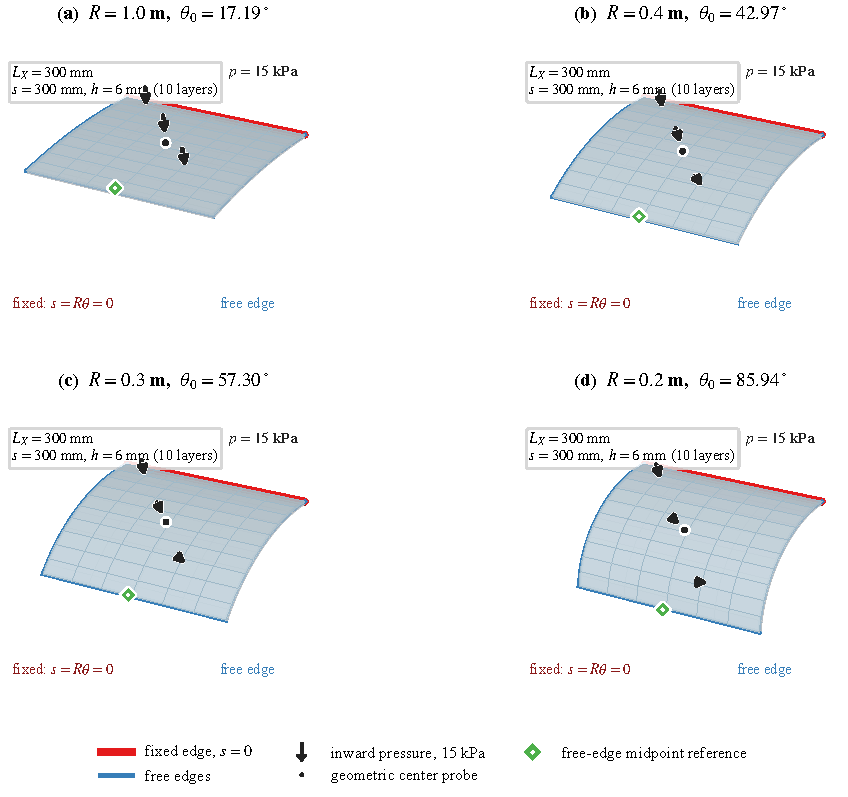
\includegraphics[width=0.92\textwidth]{figures/four_radius_geometry.pdf}
\caption{四个半径的圆柱壳几何、固定边、自由边、压力方向和中心探针。弧长保持 300~mm，半径越小，圆心角越大。}
\label{fig:four-radii}
\end{figure}

两种分布、三类载荷和两级网格共得到 48 次求解，并组成 24 组 $20\times20$ 与 $30\times30$ 配对。网格变化按 $30\times30$ 结果归一化。全部求解的机械--热残差和传感块残差均低于 $10^{-8}$。表\ref{tab:mesh}列出每个半径六种载荷--分布组合中的最大变化。

\begin{table}[H]
\centering
\caption{不同半径下中心位移的最大网格变化}
\label{tab:mesh}
\small
\begin{tabular}{rrrr}
\toprule
$R$/m & $1/R$/m$^{-1}$ & 配对数 & 最大变化/\% \\
\midrule
1.0 & 1.000 & 6 & 0.007878 \\
0.4 & 2.500 & 6 & 0.005859 \\
0.3 & 3.333 & 6 & 0.005349 \\
0.2 & 5.000 & 6 & 0.004638 \\
\bottomrule
\end{tabular}
\end{table}

24 组配对的最大变化为 0.007878\%，远低于 0.5\% 的判据。重新计算结果与旧表11中心位移的最大差为 $1.69\times10^{-13}$\%，说明旧表中的位移数值可以保留；新结果的价值在于补充了求解版本、残差和计算状态。电致与磁致工况使用同一个线性机械算子，且两种等效载荷近似成比例，因此两者相近的网格变化不能当作两次独立的机械验证。

\section{曲壳 COMSOL 目前只支持代表工况}

现有曲壳 COMSOL 结果只覆盖 $R=0.4$~m、U 分布和 15~kPa 压力。$10\times10$、$15\times15$ 和 $20\times20$ 面内网格的中心位移分别为 $-1.986667$、$-2.098474$ 和 $-2.118728$~mm；最后两级网格的变化为 0.965135\%。同一工况的 MATLAB $20\times20$ 结果为 $-1.960279$~mm，与 COMSOL 相差 8.082964\%。两者符号和量级一致，但差值明显大于位移反推中的 1.84\%。

这项比较还不能代表表11。现有 COMSOL 模型没有十个独立材料层域，没有 X 分布，也没有曲壳电致和磁致载荷；面内网格只计算到 $20\times20$。完整对照需要覆盖 4 个半径、2 种分布、3 类载荷和 2 级网格，共 48 次 COMSOL 求解。在这些工况完成之前，代表工况只能用于观察模型形式差异，不能用于判断表11全部数据的跨软件精度。

\section{结论}

逐层源项装配修正解决了位移反推中的重复累加问题。修正后的电势和磁势与 COMSOL 相差约 1.84\%，说明两套非同构实现给出了相近的线性响应。曲壳表11的 24 组 MATLAB 位移已经通过 $20\times20$ 到 $30\times30$ 的网格检查，最大变化为 0.007878\%。目前只有一个曲壳压力工况完成 COMSOL 比较，因此完整的表11跨软件验证仍缺少其余工况。

\end{document}

